% ============================================================
%  Altar Valley Berms — Figure Summary  (Paper 1)
%  Paper 1: Berm condition and vegetation response
%  Captions drawn from figures/paper1/figure_registry_concise.txt
%  Date: 2026-03-01
% ============================================================
\documentclass[11pt, a4paper]{article}

\usepackage[utf8]{inputenc}
\usepackage[T1]{fontenc}
\usepackage{lmodern}
\usepackage[left=2.5cm, right=2.5cm, top=2.5cm, bottom=2.5cm]{geometry}
\usepackage{graphicx}
\usepackage{caption}
\usepackage{float}
\usepackage{parskip}
\usepackage{microtype}
\usepackage{hyperref}
\hypersetup{colorlinks=true, linkcolor=black, urlcolor=blue}

% ── compact figure caption style ─────────────────────────────
\captionsetup{font=small, labelfont=bf, justification=raggedright, singlelinecheck=false}

% ============================================================
\begin{document}

\begin{center}
  {\LARGE \textbf{Geomorphic and Soil Controls on Berm Structural Integrity}} \\
  {\LARGE \textbf{and Vegetation Response in the Altar Valley, Arizona}} \\[0.4em]
  {\large Figure Summary — Paper 1} \\[0.3em]
  {\small Generated 2026-03-01 \quad|\quad Source: \texttt{figures/paper1/figure\_registry\_concise.txt}}
\end{center}

\vspace{1em}
\hrule
\vspace{1.5em}

% ── Figure 1 ─────────────────────────────────────────────────
\begin{figure}[H]
  \centering
  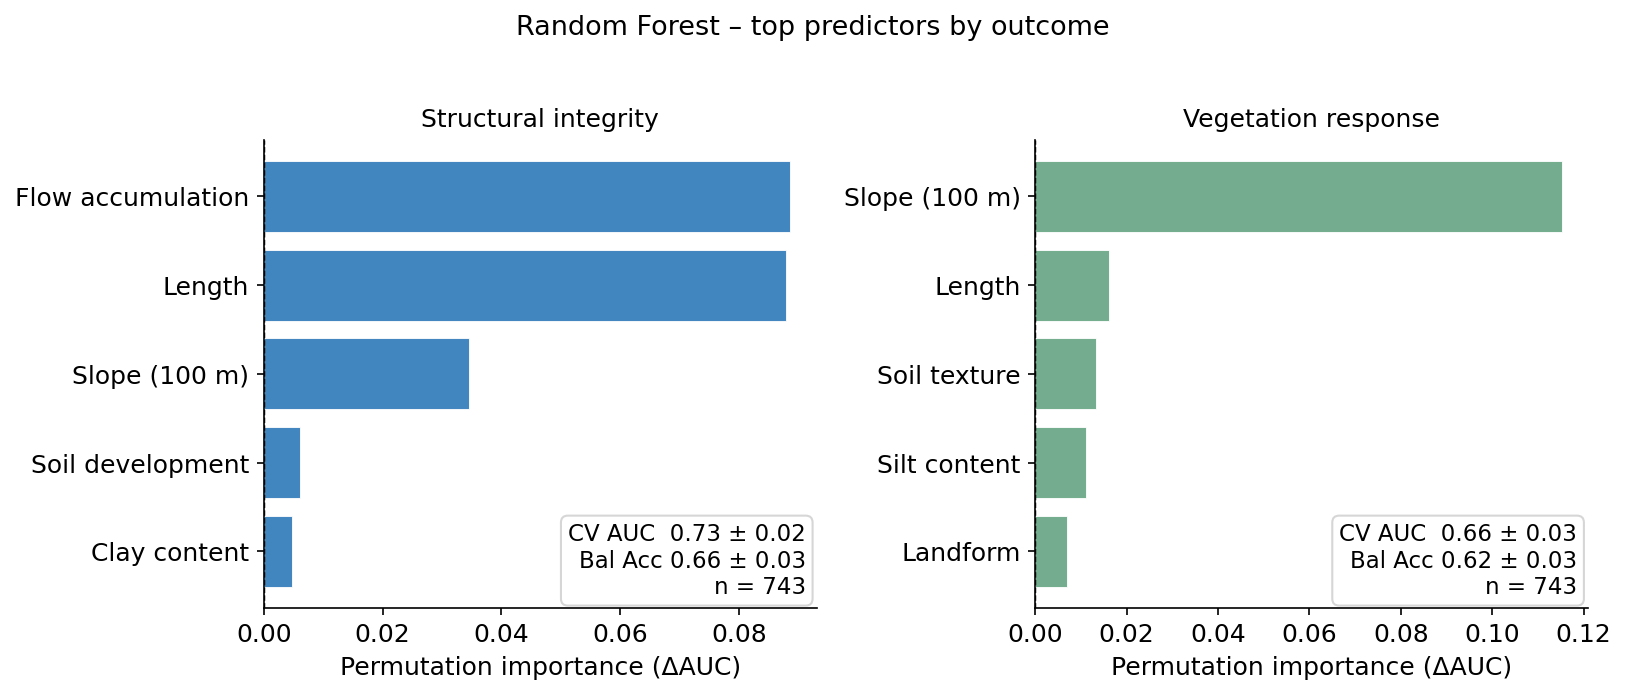
\includegraphics[width=\linewidth]{../figures/paper1/fig1_rf_permutation_importance.png}
  \caption*{\textbf{Figure 1.}
    Random Forest classifier with 5-fold cross-validation; permutation importance
    computed by randomly shuffling each predictor and measuring the decrease in AUC.
    Top 5 predictors shown for each outcome.
    The top predictors for structural integrity are flow accumulation, berm length,
    slope (100\,m and 200\,m), and soil texture.
    For vegetation response, the top predictors are landform, soil texture, flow
    accumulation, soil development, and berm length.
    Both outcomes are strongly associated with berm length and landscape position
    (flow accumulation), while vegetation response is more influenced by soil and
    landform characteristics than structural integrity.}
\end{figure}

\vspace{2em}

% ── Figure 1 (alternate) ─────────────────────────────────────
\begin{figure}[H]
  \centering
  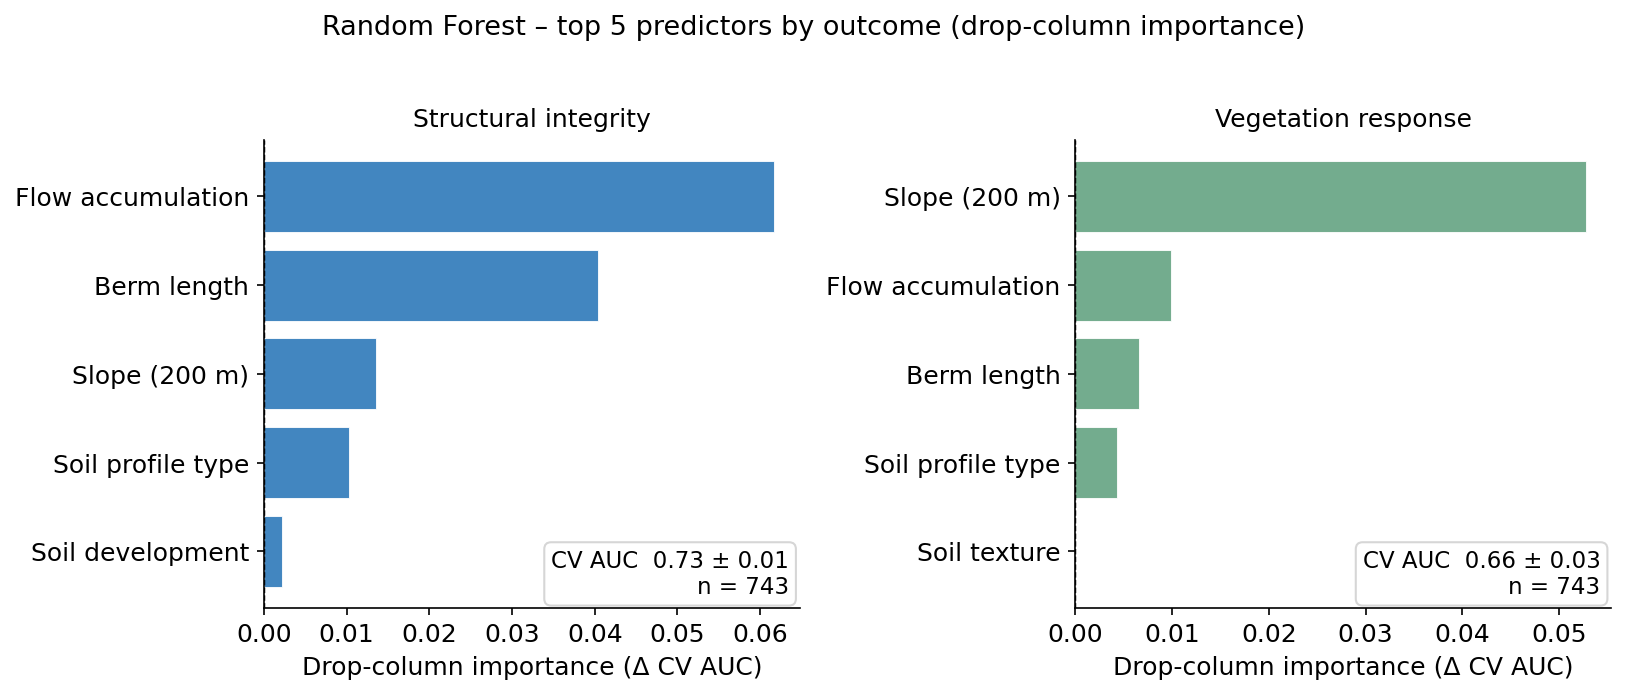
\includegraphics[width=\linewidth]{../figures/paper1/fig1_alt.png}
  \caption*{\textbf{Figure 1 (alternate).}
    Random Forest classifier with 5-fold cross-validation; drop-column importance
    computed by comparing baseline CV AUC (with all predictors) to CV AUC with
    each predictor removed. Top 5 predictors shown for each outcome.
    The top predictors for structural integrity are berm length, slope (200\,m),
    slope (100\,m), flow accumulation, and soil texture.
    For vegetation response, the top predictors are landform, soil texture, flow
    accumulation, berm length, and soil development.
    Both outcomes show strong associations with berm length and landscape position
    (flow accumulation), while vegetation response is more strongly influenced by
    soil and landform characteristics.}
\end{figure}

\clearpage

% ── Figure 2 ─────────────────────────────────────────────────
\begin{figure}[H]
  \centering
  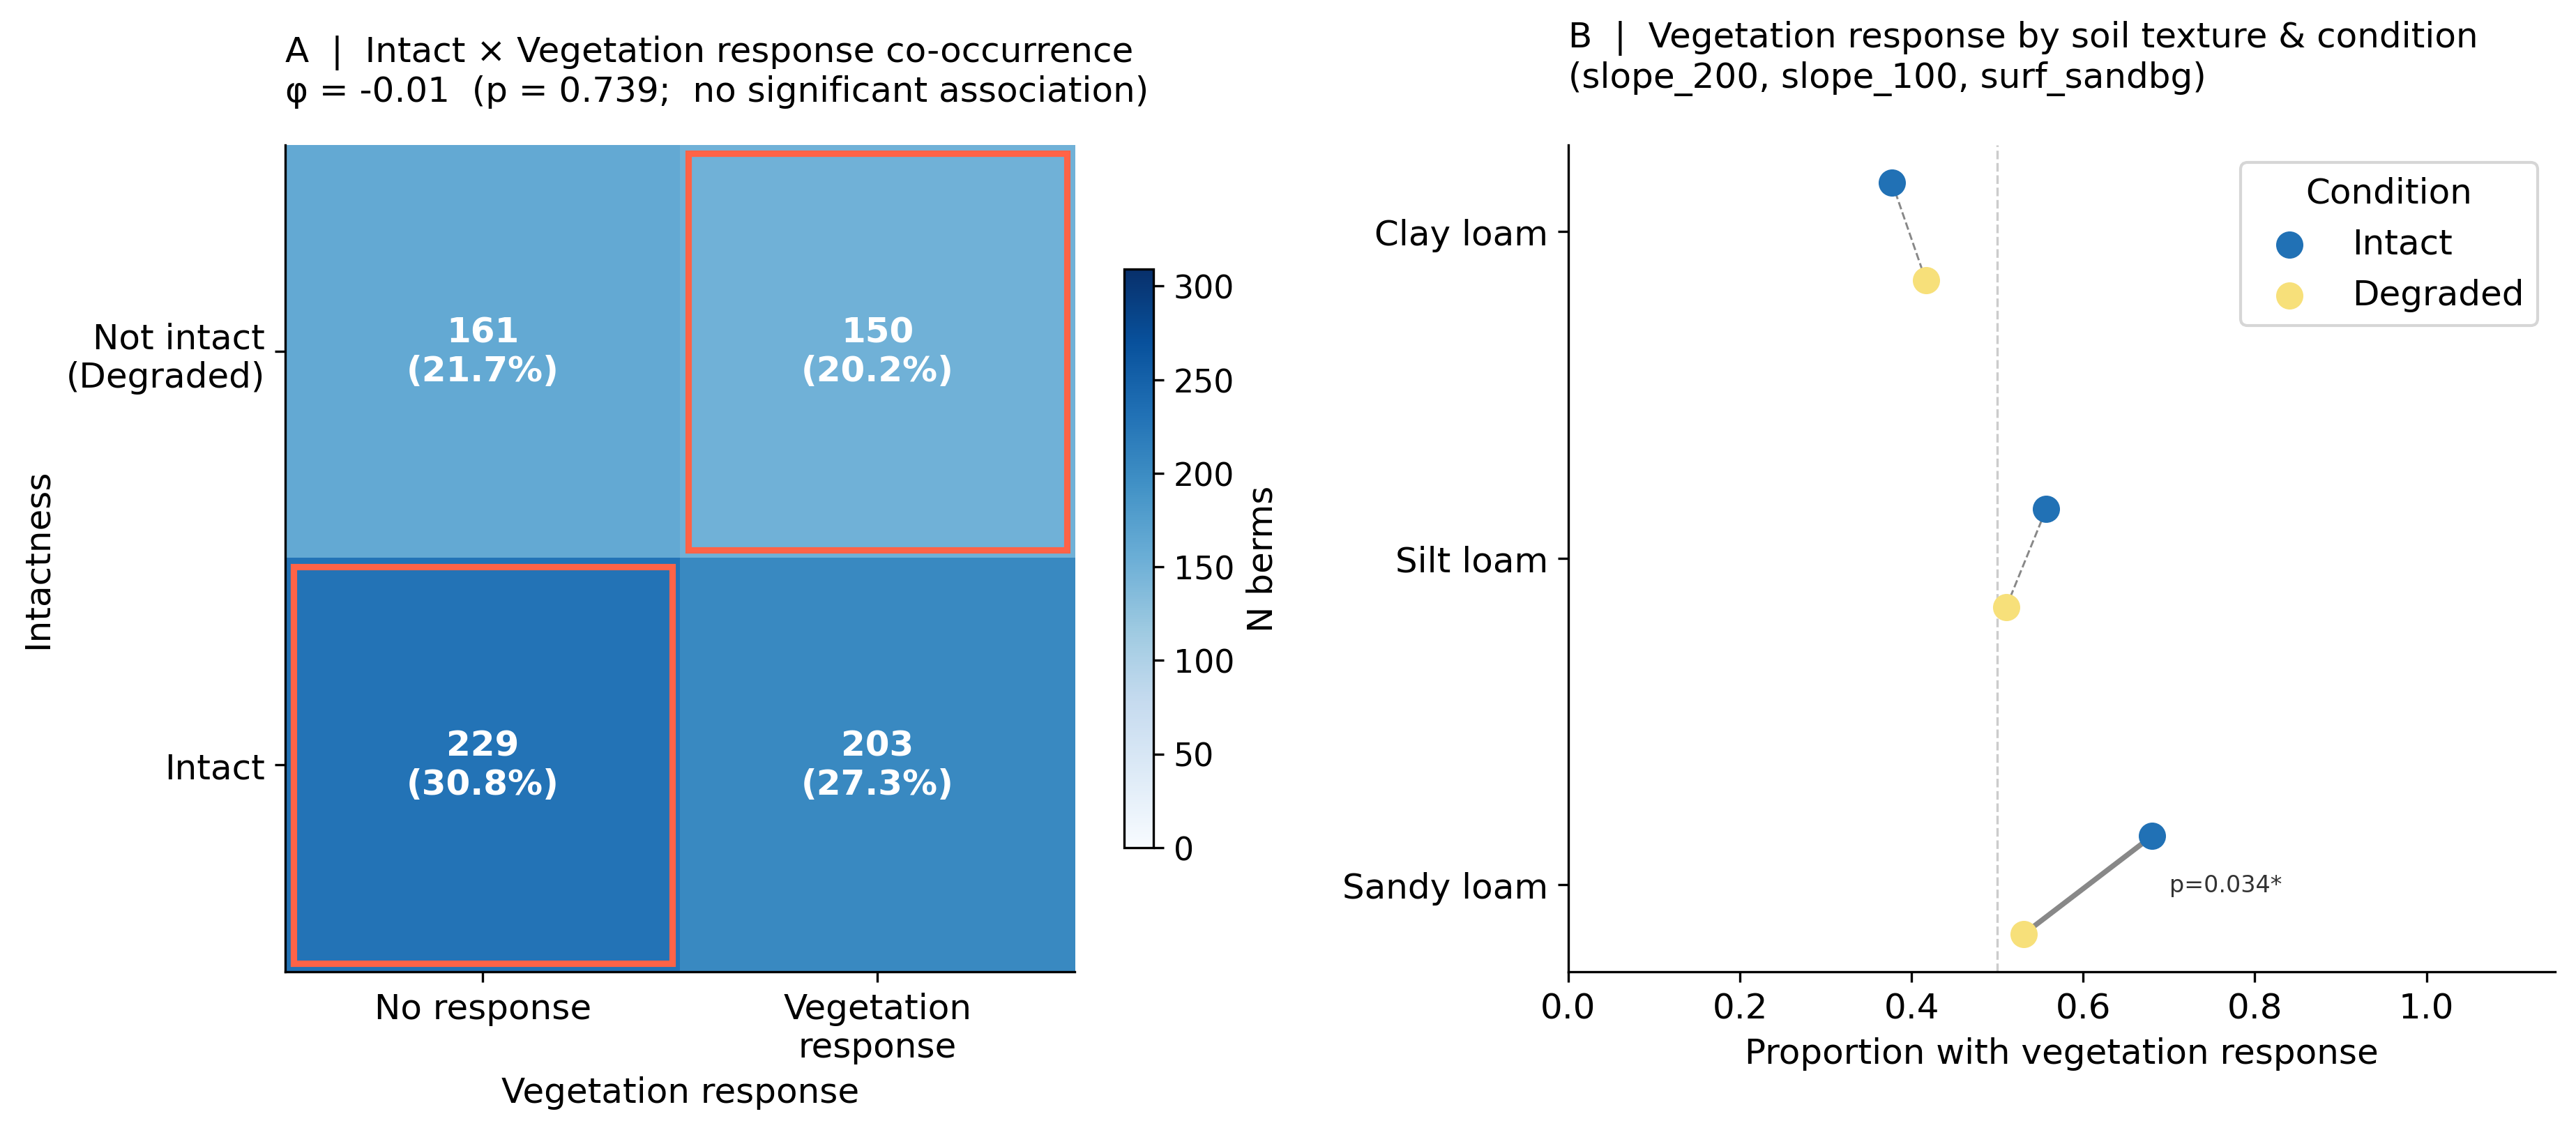
\includegraphics[width=\linewidth]{../figures/paper1/fig2_geomorph_soil_intact_effective.png}
  \caption*{\textbf{Figure 2.}
    Panel A uses Pearson $\chi^2$ ($\varphi$ coefficient) for a 2$\times$2
    intact $\times$ vegetation-response table; Panel B uses two-sided Fisher's
    exact test to compare proportions between Intact and Degraded berms within
    each soil texture class.
    Berm intactness and vegetation response are statistically independent
    ($\varphi = -0.01$, $p = 0.739$), indicating that intact and degraded berms
    produce vegetation responses at similar overall rates.
    The exception is Sandy loam, where intact berms show significantly higher
    vegetation response than degraded berms ($p = 0.034$).}
\end{figure}

\vspace{2em}

% ── Figure 3 ─────────────────────────────────────────────────
\begin{figure}[H]
  \centering
  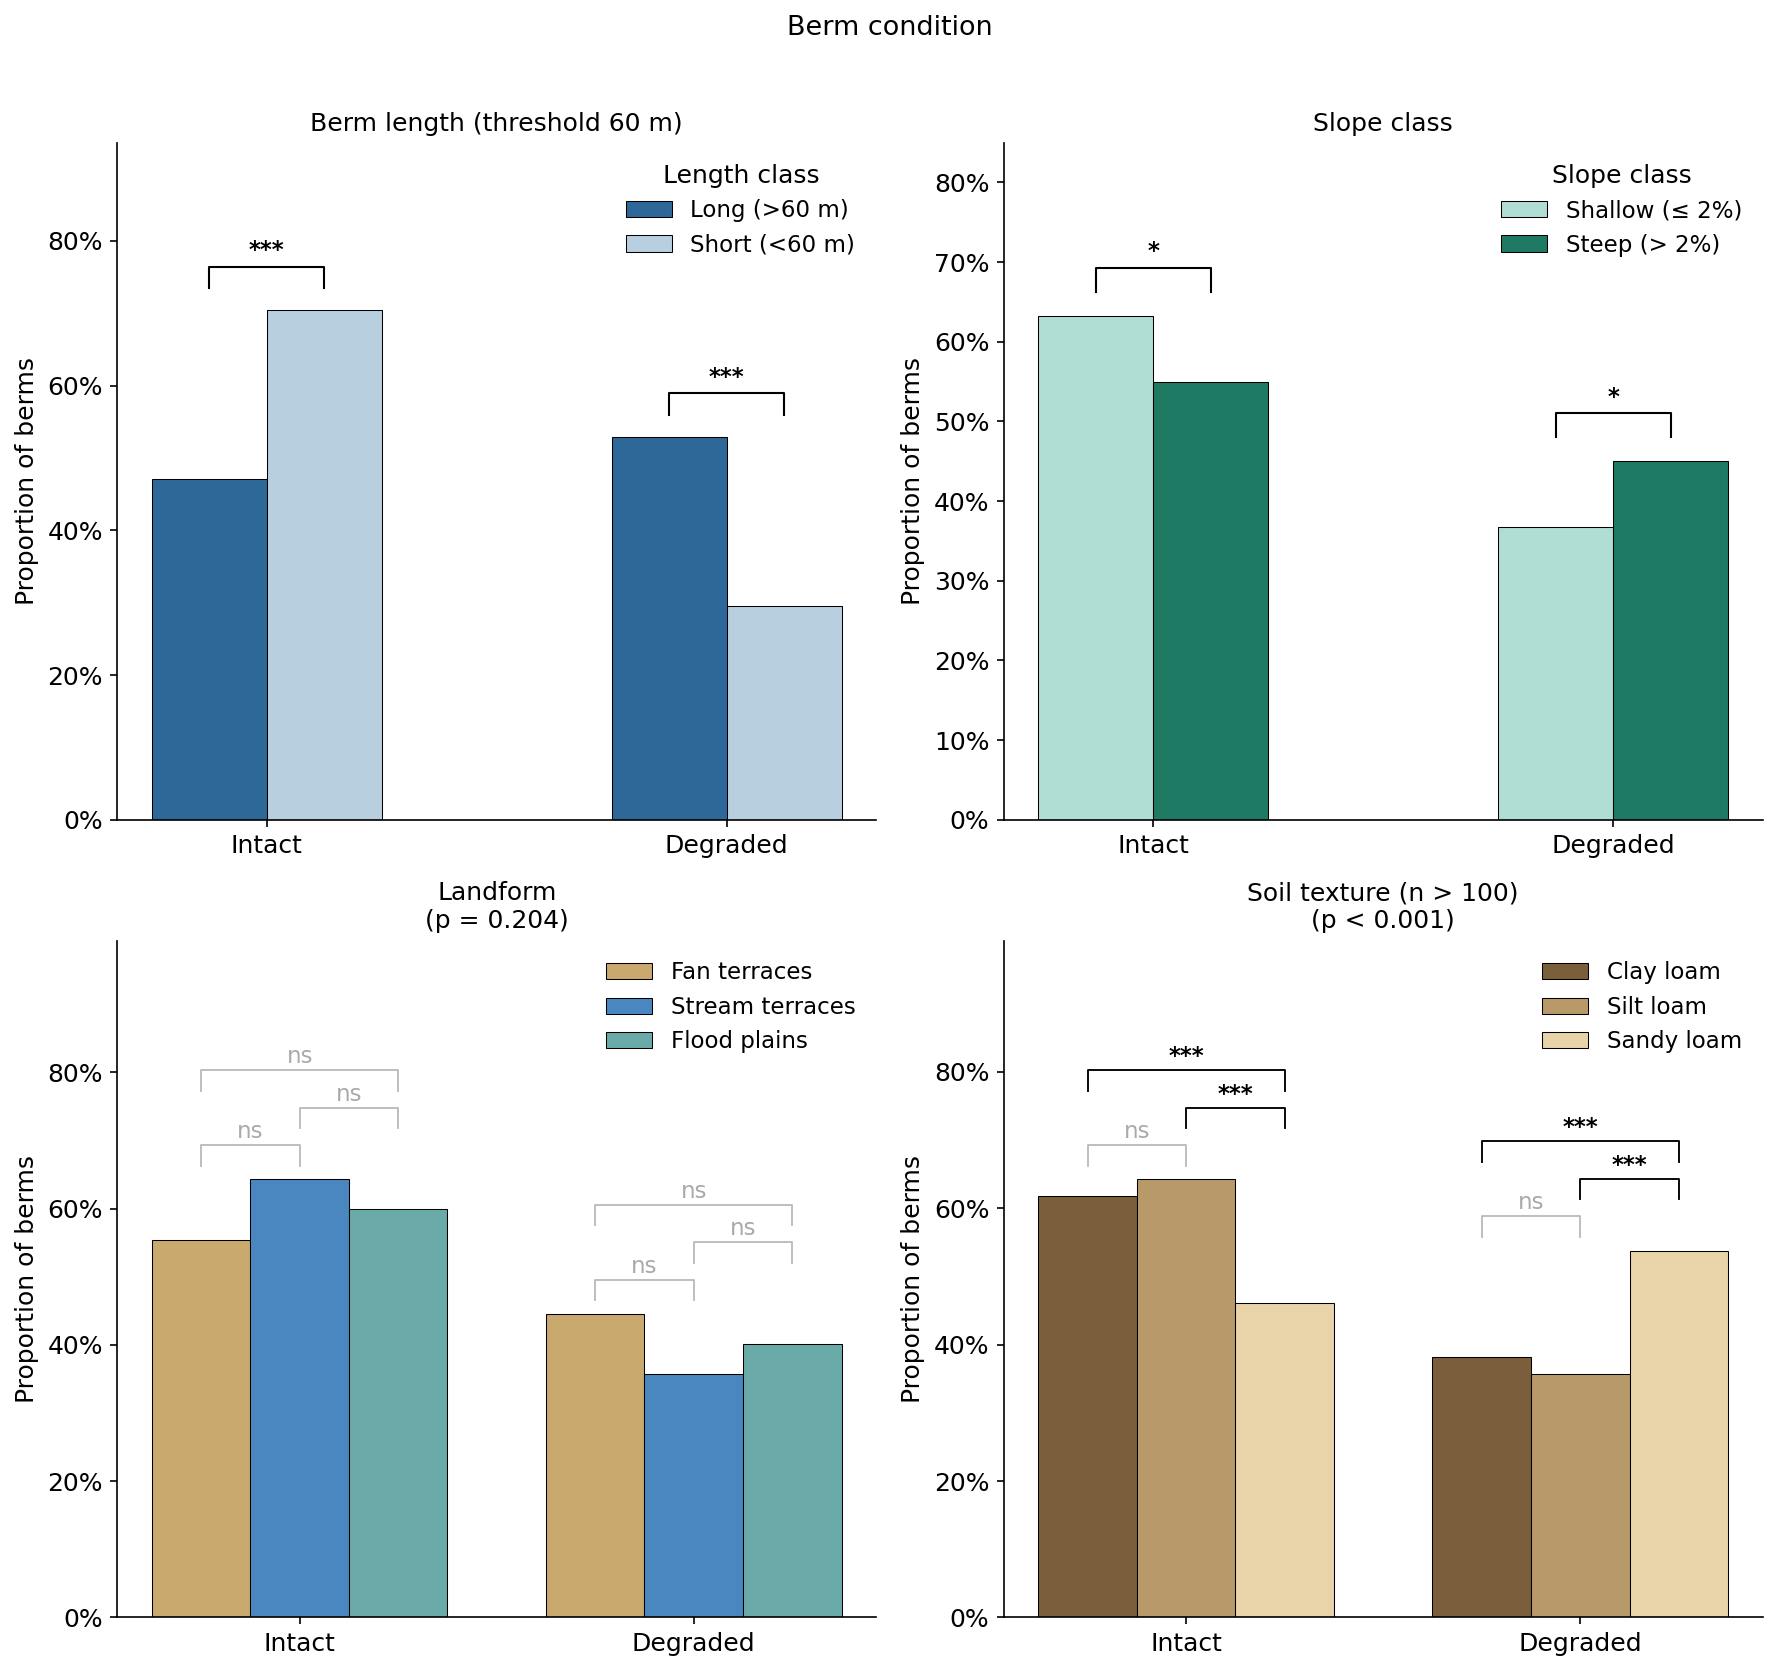
\includegraphics[width=\linewidth]{../figures/paper1/fig3_berm_condition.png}
  \caption*{\textbf{Figure 3.}
    Two-category panels use one-sided Fisher's exact test; multi-category panels
    (landform, texture) use pairwise Fisher's exact with overall $\chi^2$ $p$-value.
    Berm condition is strongly associated with berm length~--- shorter berms are
    markedly more likely to be intact ($p < 0.001$)~--- and modestly associated
    with slope class ($p < 0.05$).
    Landform does not significantly predict condition ($p = 0.204$), but soil
    texture does ($p < 0.001$).}
\end{figure}

\clearpage

% ── Figure 4 ─────────────────────────────────────────────────
\begin{figure}[H]
  \centering
  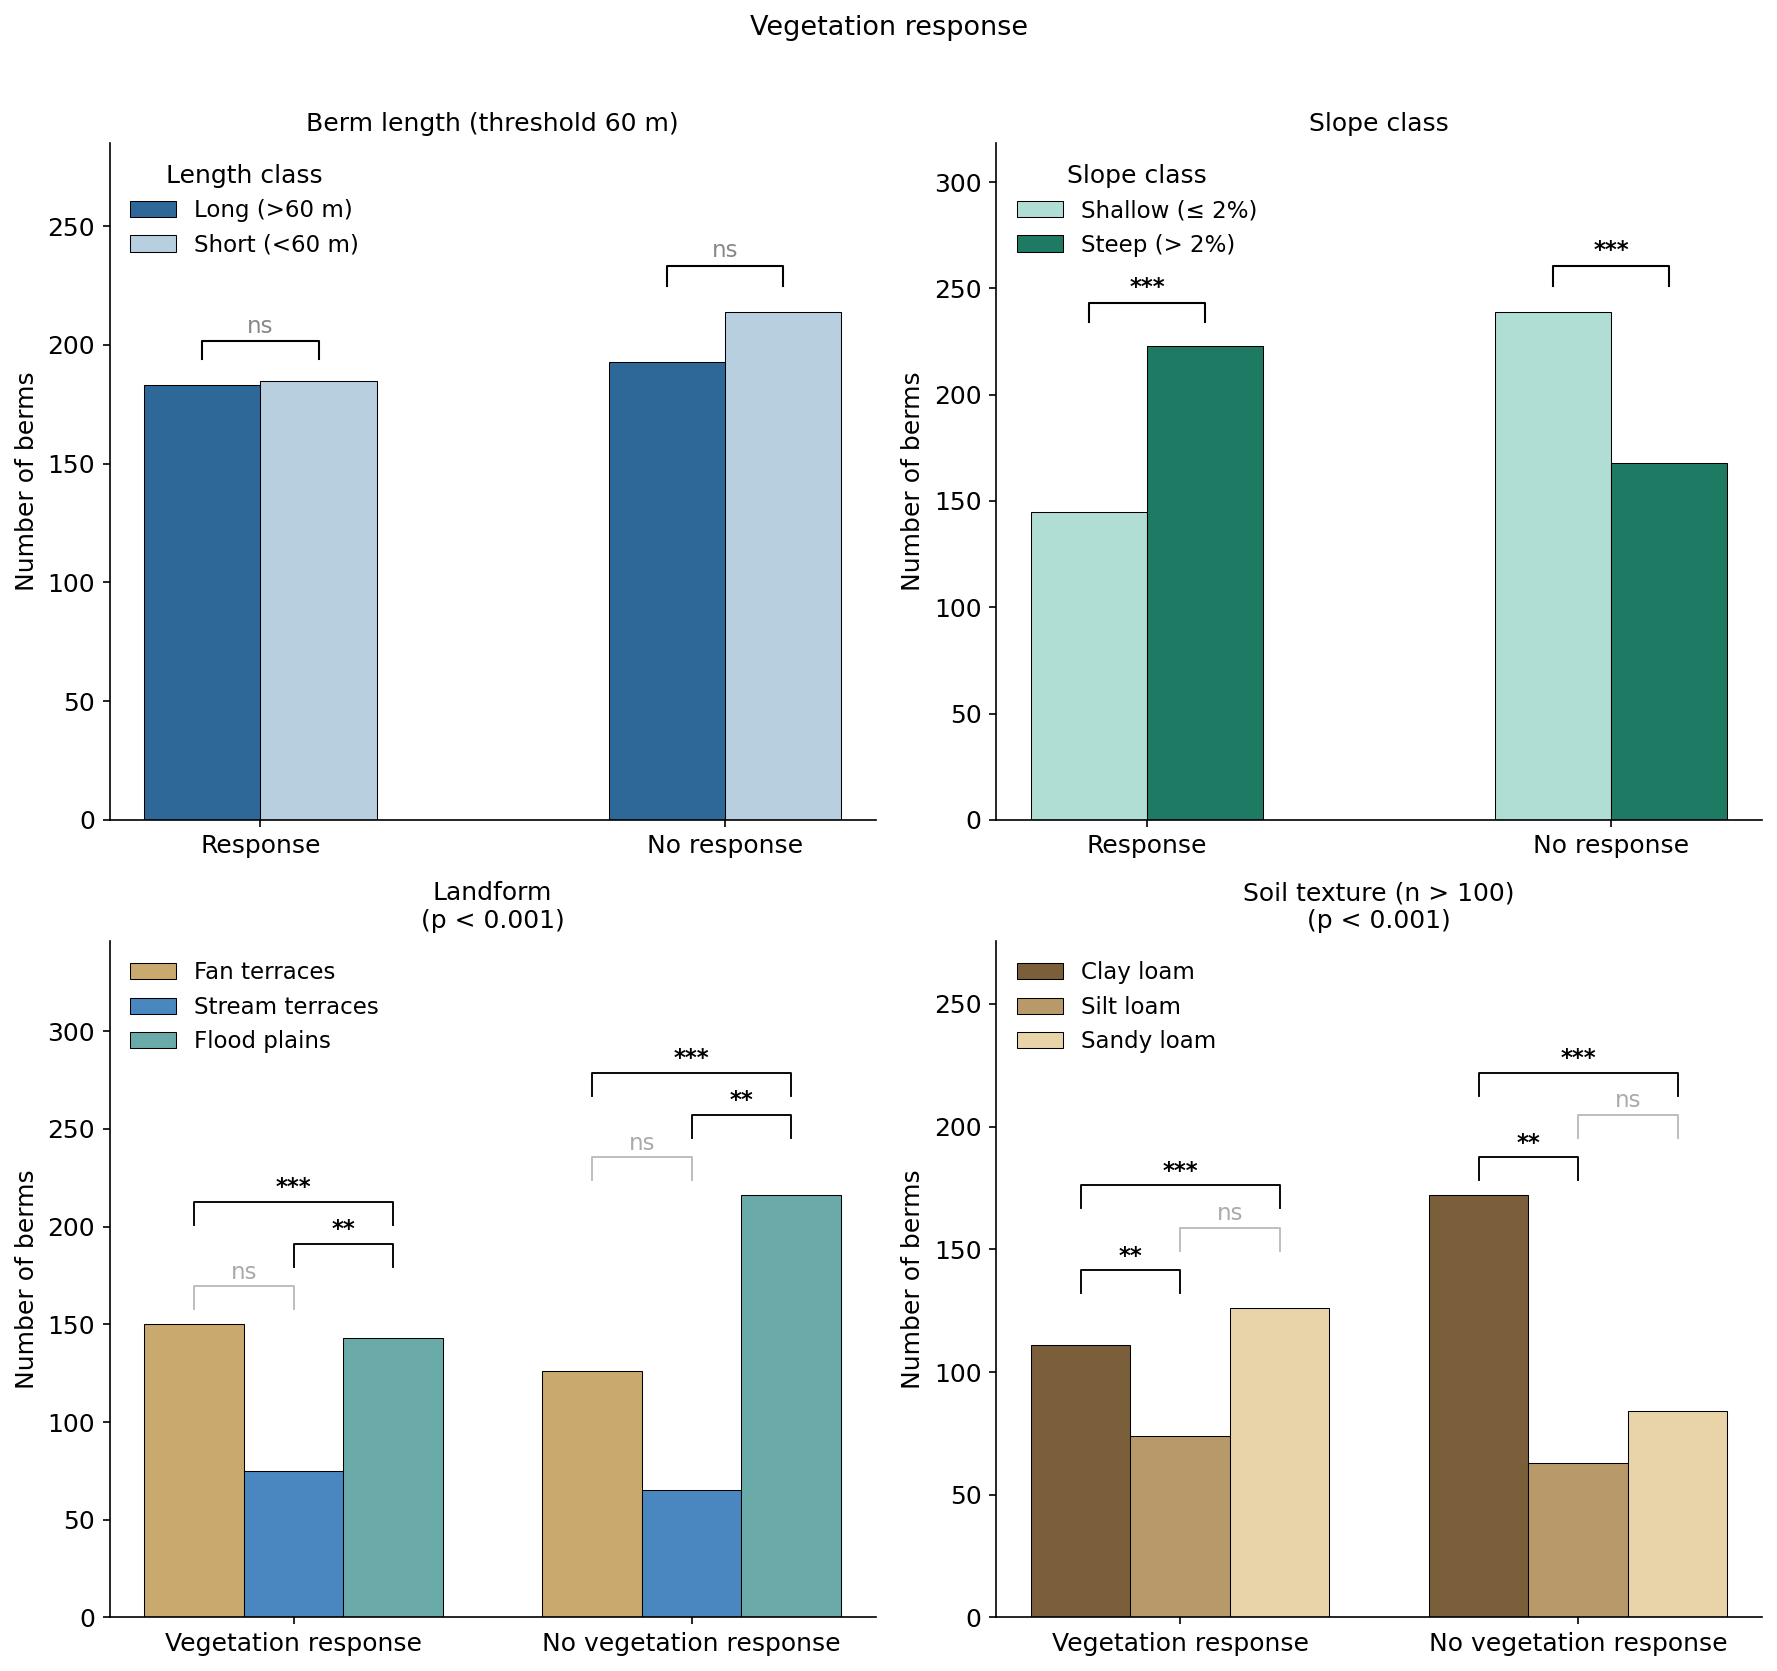
\includegraphics[width=\linewidth]{../figures/paper1/fig4_vegetation_response.png}
  \caption*{\textbf{Figure 4.}
    Two-category panels use one-sided Fisher's exact test; multi-category panels
    (landform, texture) use pairwise Fisher's exact with overall $\chi^2$ $p$-value.
    Vegetation response is significantly associated with slope class ($p < 0.001$),
    landform ($p < 0.001$), and soil texture ($p < 0.001$), but not with berm
    length alone.
    Steep-slope berms and flood-plain berms show the highest rates of vegetation
    response.}
\end{figure}

\clearpage

% ── Supplementary Figure 1 ───────────────────────────────────
\begin{figure}[H]
  \centering
  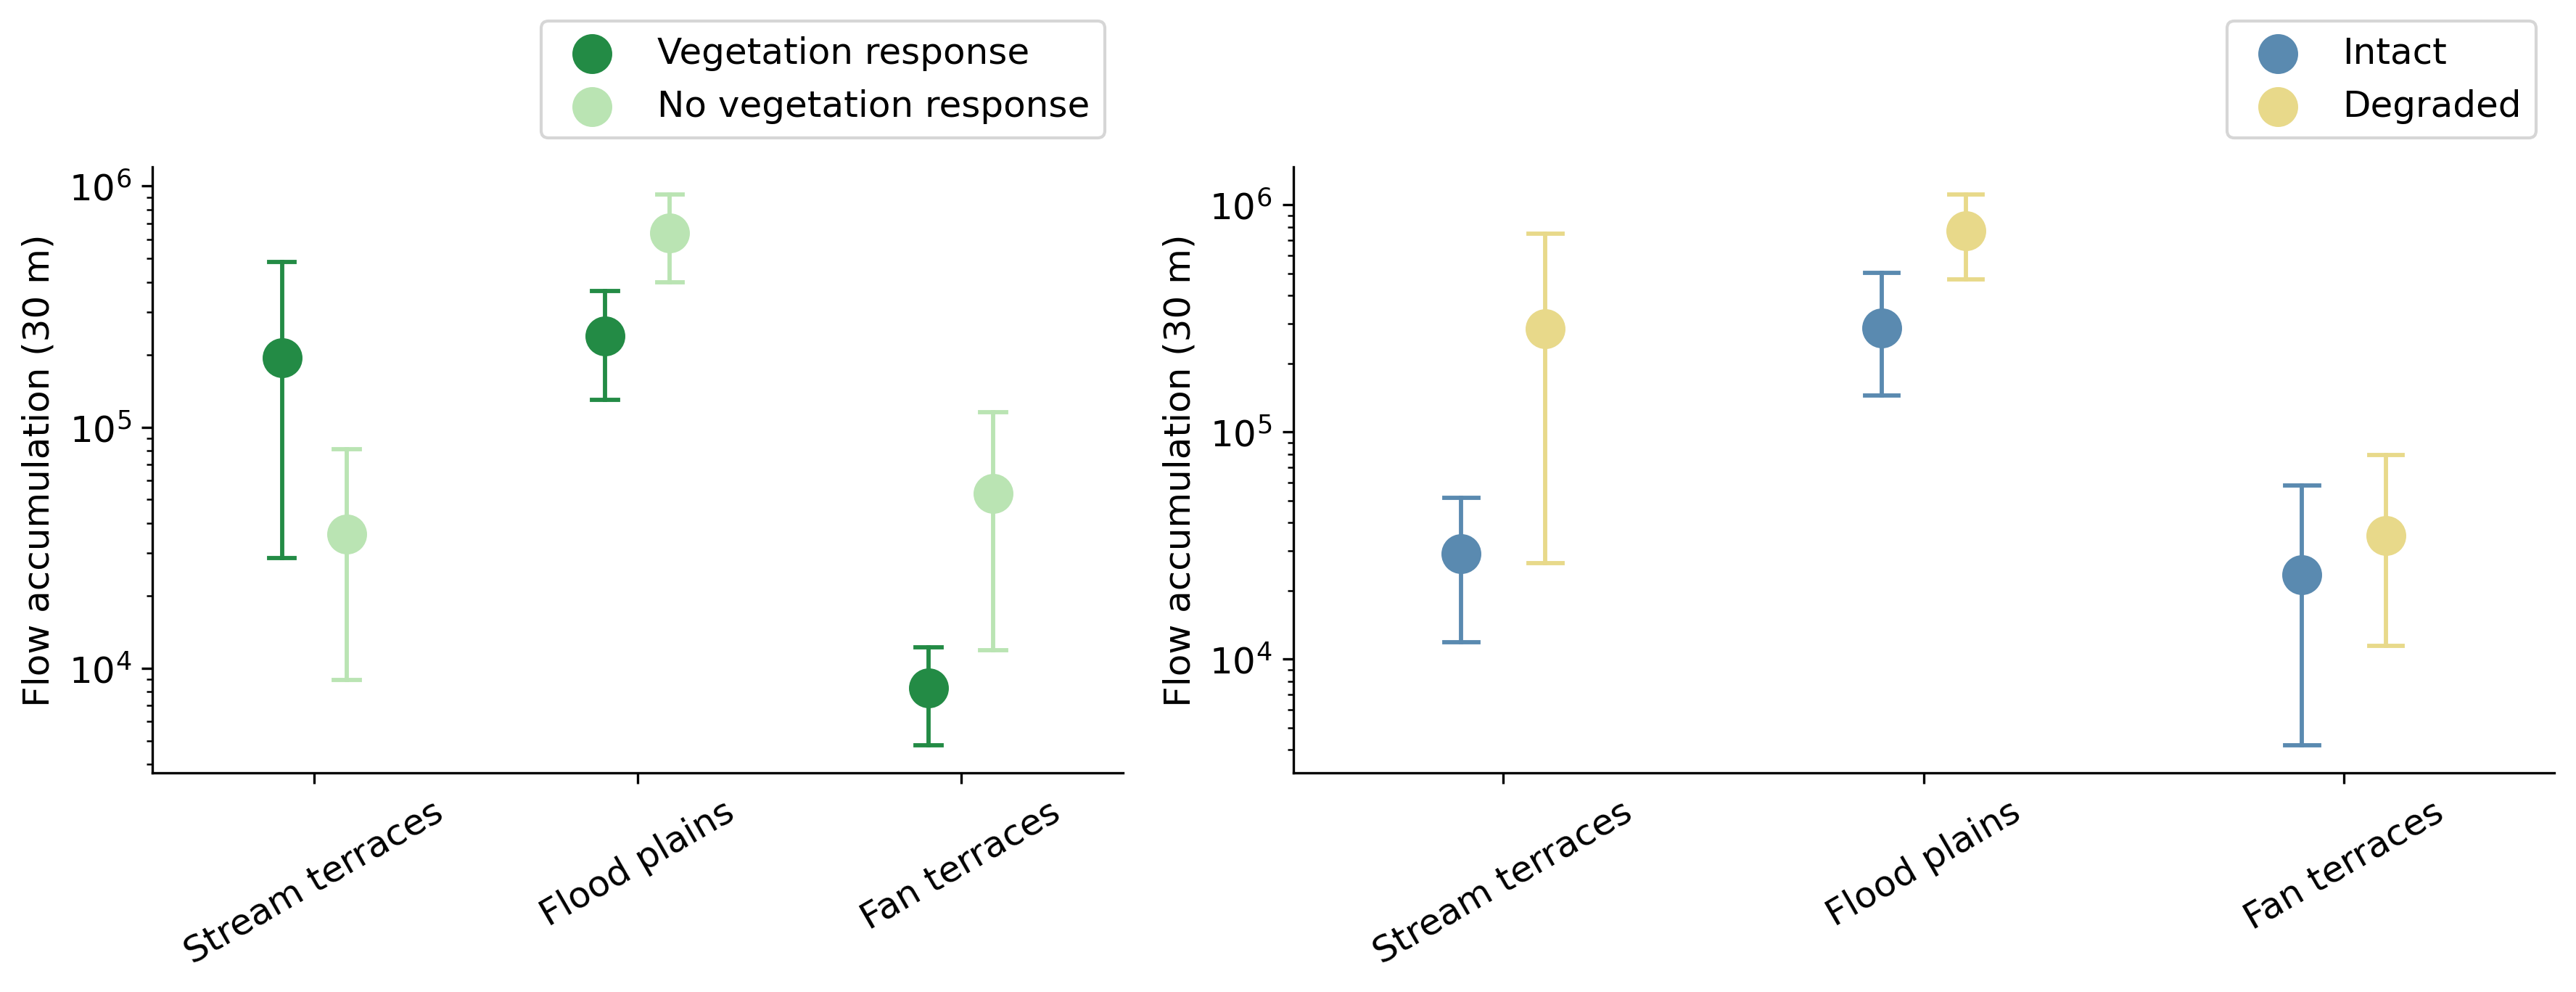
\includegraphics[width=\linewidth]{../figures/paper1/SI_fig1_fa30_pointplot_by_landform.png}
  \caption*{\textbf{Supplementary Figure 1.}
    Point plots show mean $\pm$ 95\,\% CI of 30\,m flow accumulation (log scale)
    by landform, grouped by vegetation response (Panel A) and structural condition
    (Panel B).
    Flood-plain berms experience the highest contributing flow accumulation
    regardless of outcome, while fan-terrace berms receive the least.
    Within each landform, effective berms tend to have similar or higher flow
    accumulation than ineffective berms, and degraded berms tend toward higher
    values than intact berms, consistent with greater hydraulic stress on degraded
    structures.}
\end{figure}

\vspace{2em}

% ── Supplementary Figure 2 ───────────────────────────────────
\begin{figure}[H]
  \centering
  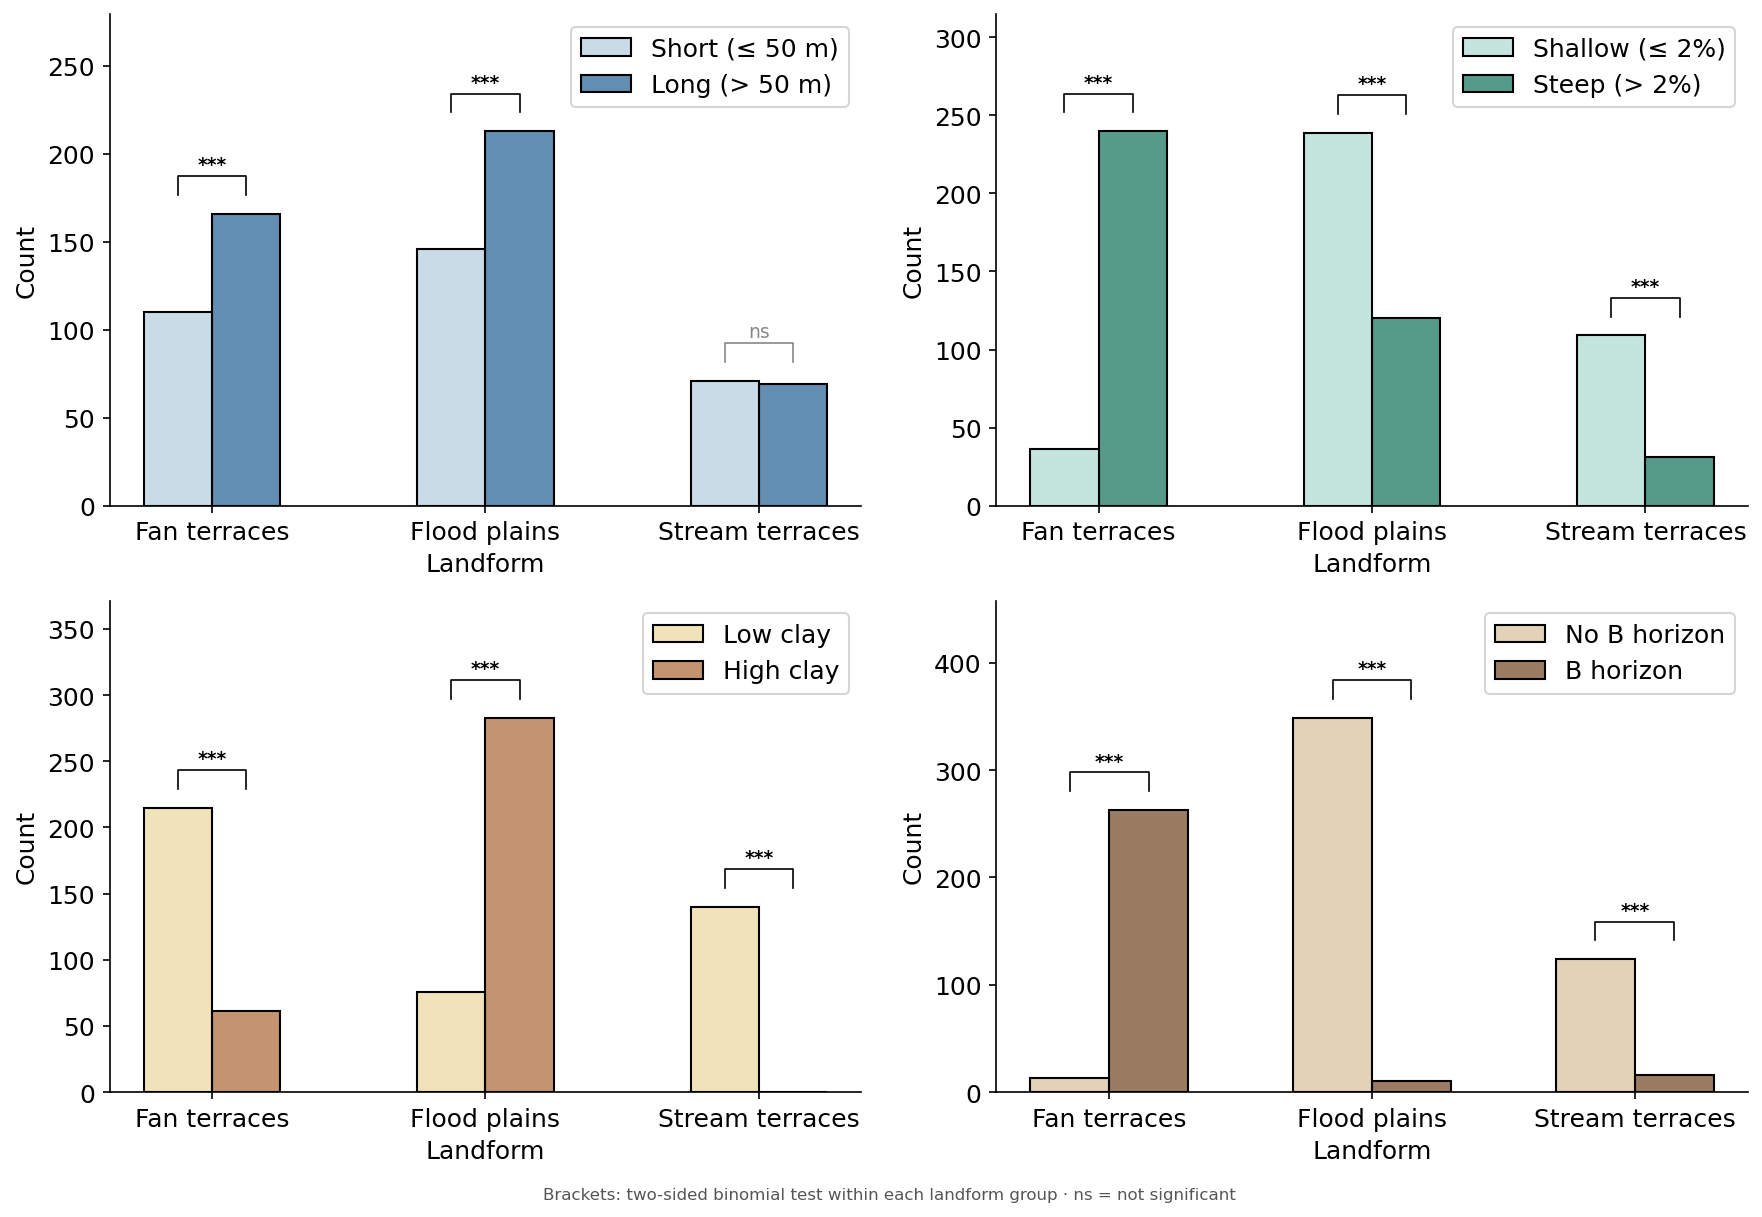
\includegraphics[width=\linewidth]{../figures/paper1/SI_landform_by_predictors.png}
  \caption*{\textbf{Supplementary Figure 2.}
    Two-sided binomial test ($H_0$: 50/50 split) applied within each landform
    group for each predictor category (length, slope, clay content, soil
    development); labels: *** $p < 0.001$, ** $p < 0.01$, * $p < 0.05$,
    ns~$p \geq 0.05$.
    Predictors are non-randomly distributed across landforms~--- high-clay soils
    concentrate on flood plains, steep slopes on fan terraces, and B-horizon
    development on fan and stream terraces~--- confirming that landform is a
    meaningful stratification variable and motivating its inclusion as a covariate.}
\end{figure}

\clearpage

% ── Supplementary Figure 3 ───────────────────────────────────
\begin{figure}[H]
  \centering
  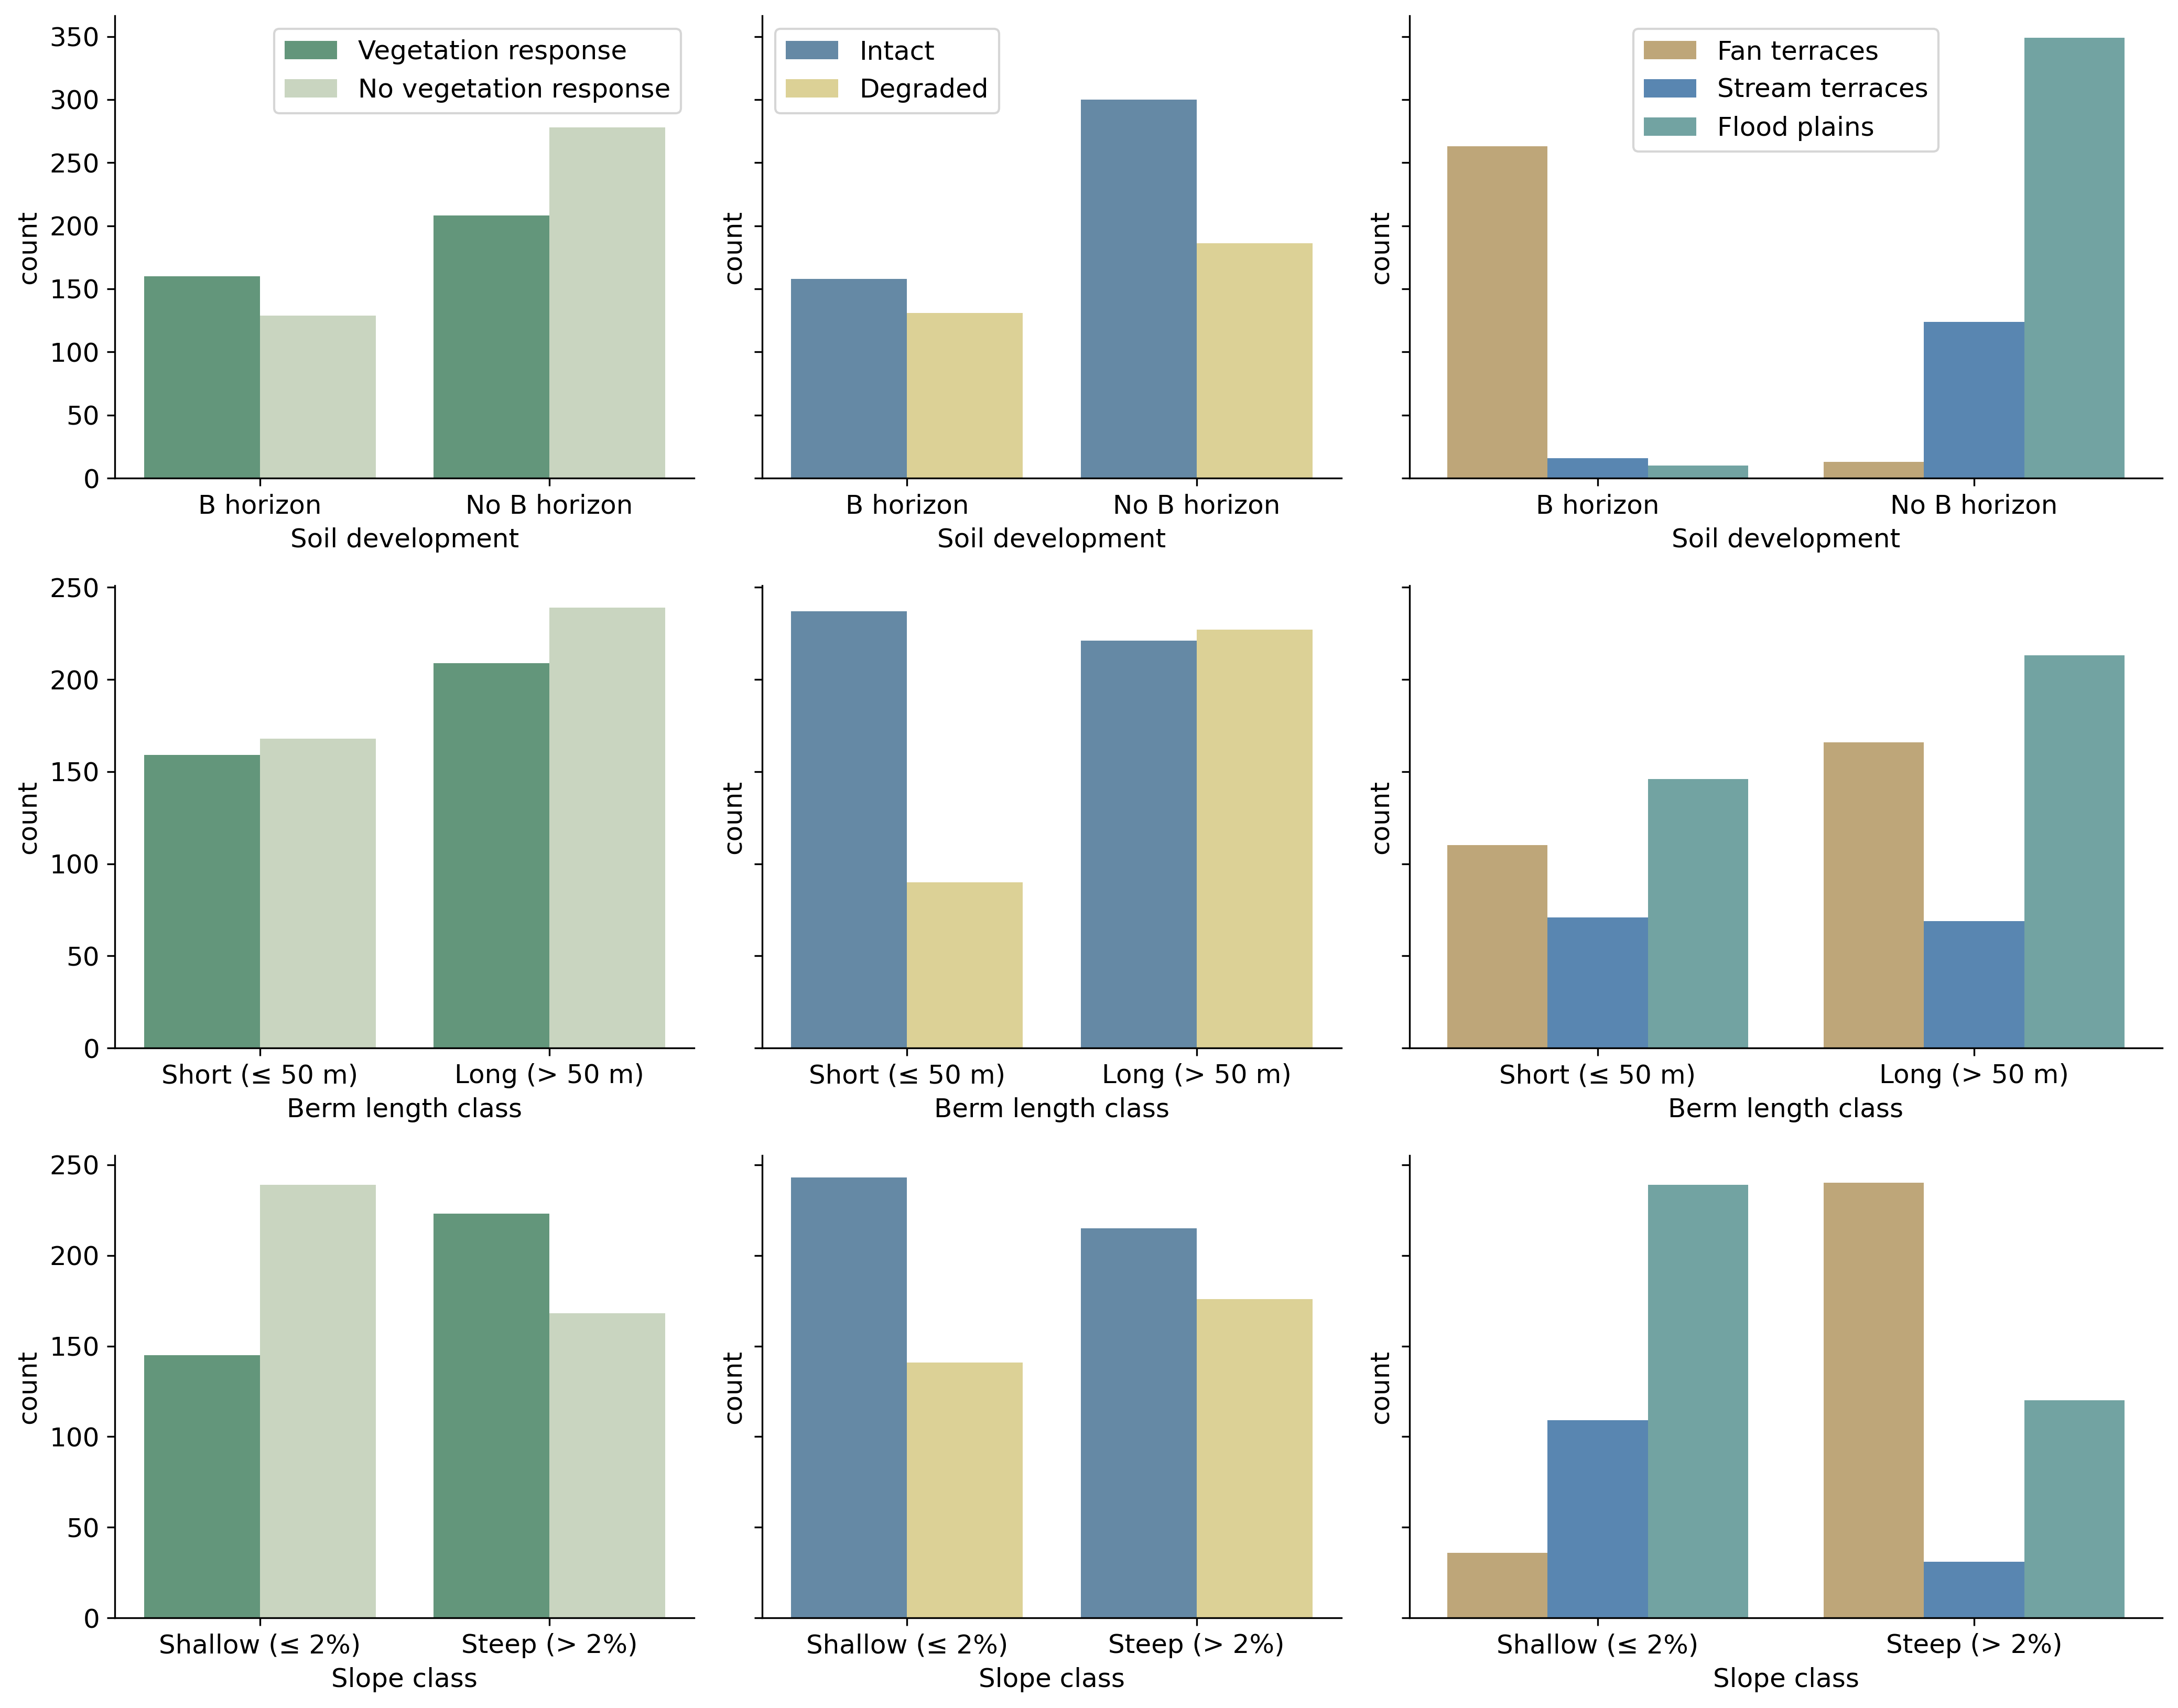
\includegraphics[width=\linewidth]{../figures/paper1/SI_fig3_countplots_by_outcome_and_landform.png}
  \caption*{\textbf{Supplementary Figure 3.}
    $3 \times 3$ panel of count plots.
    Rows: soil development (B horizon vs.\ none), berm length class (short
    vs.\ long), slope class (shallow vs.\ steep).
    Columns: vegetation response, structural condition, landform.
    Fan-terrace berms are overwhelmingly found in B-horizon soils, whereas
    stream-terrace and flood-plain berms dominate in soils without a B horizon.
    Berm length and slope class are more evenly distributed across outcomes,
    though short berms are disproportionately intact and steep-slope berms show
    a higher proportion of vegetation response.}
\end{figure}

\end{document}
